\documentclass{astroedu-lab}

\begin{document}

\pagestyle{plain}

\begin{problem}{\huge Лабораторная работа 5.5.1\\\\Измерение коэффициента\\\\ослабления потока $\gamma$-лучей\\\\в веществе\\\\Выполнил Жданов Елисей Б01-205}

\section{Цель работы:}

С помощью сцинтилляционного счётчика измеряются линейные коэффициенты ослабления потока $\gamma$-лушче в свинце, железе и алюминии; по их величине определяется энергия $\gamma$-квантов.

\section{Оборудование:}

Источник излучения

$\gamma$ спектрометр

\section{Теоретическая справка}

Проходя через вещество, пучок $\gamma$-квантов постепенно ослабляется, ослабление происходит по экспоненциальному закону, который может быть записан в двух эквивалентных формах:
\[\begin{array}{l}
I = I_0 e^{-\mu l} ,\\
I = I_0 e^{-\mu' m_l},\\
\end{array}\]
где $I, I_0$ -- интенсивности прошедшего и падающего излучений, $l$ -- длина пути, пройденного пучком $\gamma$-лучей, $m_l$ -- масса пройденного вещества на единицу площади, $\mu$, $\mu'$ -- константы, зависящие от вещества. Ослабление потока $\gamma$-лучей возникает из-за фотоэлектрического поглощения, комптоновского рассеяния и генерации электрон-позитронных пар (при достаточных энергиях).\\
Считая геометрию идеальной, то есть сквозь вещество всегда идёт узкий параллельный пучок, можно считать, что комптоновское рассеяние выводит $\gamma$-кванты из пучка и в итоге меняется количество, но не энергия $\gamma$-квантов. Это означает, что $\mu$ не зависит от $l$. Число выбывших на пути $dl$ из пучка $\gamma$-квантов
\[-dN = \mu N dl,\]
откуда
\[N = N_0 e^{\mu l},\]
или
\begin{equation}
\mu = \dfrac{1}{l} \ln \dfrac{N_0}{N}.
\end{equation}

\section{Экспериментальная установка}

\begin{figure}[h]
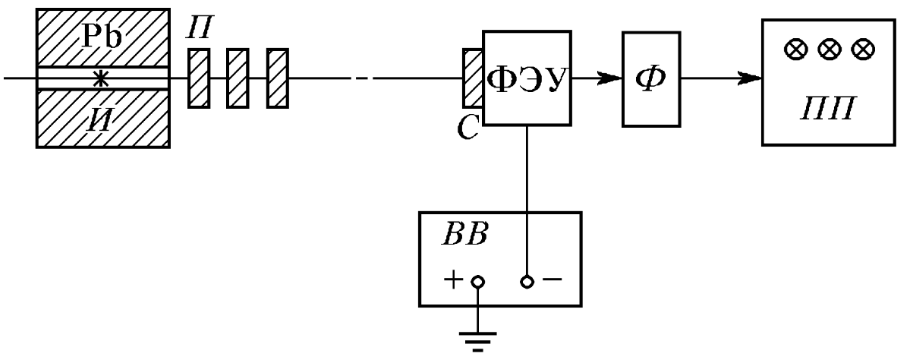
\includegraphics[scale=0.5]{1.png}
\centering
\caption{Схема установки.}
\end{figure}
На Рис. 1 изображена схема установки. Свинцовый коллиматор выделяет узкий почти параллельный пучок $\gamma$-квантов, проходящий через набор поглотителей П и регистрируемый сцинтилляционным счётчиком. Сигналы от счётчика усиливаются и регистрируются пересчётным прибором ПП. Высоковольтный выпрямитель ВВ обеспечивает питание сцинтилляционного счётчика. Чтобы уменьшить влияние плохой геометрии, счётчик расположен на большим расстоянии от источника, поглотители имеют небольшие размеры, а так же устанавливаются на расстоянии друг от друга, чтобы испытавшие комптоновское рассеяние кванты с меньшей вероятностью могли в него вернуться.

\section{Измерения, Обработка}

Включив установку, убеждаемся в том, что она чувствует гамма-лучи: подаем на ФЭУ напряжение, указанное на установке. Не забываем прогреть установку положенное время(10 минут). Измерив скорость счета при полностью открытом коллиматоре, а затем при коллиматоре, закрытом свинцовой пробкой, отметим, что скорость счета резко уменьшается (см результаты измерений), что свидетельствует об исправности счетчика. Счетчик не уходит в зашкал, проверим, что скорость счета в 1000 импульсов выполняется для всех образцов, при необходимости интервал был увеличен до 20 секунд.

Теперь исследуем поглощение $\gamma$-лучей в свинце, железе и алюминии. Для этого измеряем число частиц, попадающих в счетчик. Количество поглощенных лучей измеряем для разного числа образцов. Погрешность измерений считаем корнем из числа частиц ($\sigma_N = \sqrt{N}$).

Погрешность всех измерений толщины считаем приборной $\sigma_x = 0.2~\text{см}$.

Построим кривые зависимости логарифма посчитанных частиц $\ln N$, где $N_0$ -- число частиц без поглотителей, от суммарной толщины образцов $l$.
Погрешность N пропорциональна $\sqrt N$.

Графики представим на рисунке. Прямые имеют фиксированную точку пересечения с осями в нуле. С помощью МНК найдём коэффициент наклона прямых.

\begin{figure}[h]
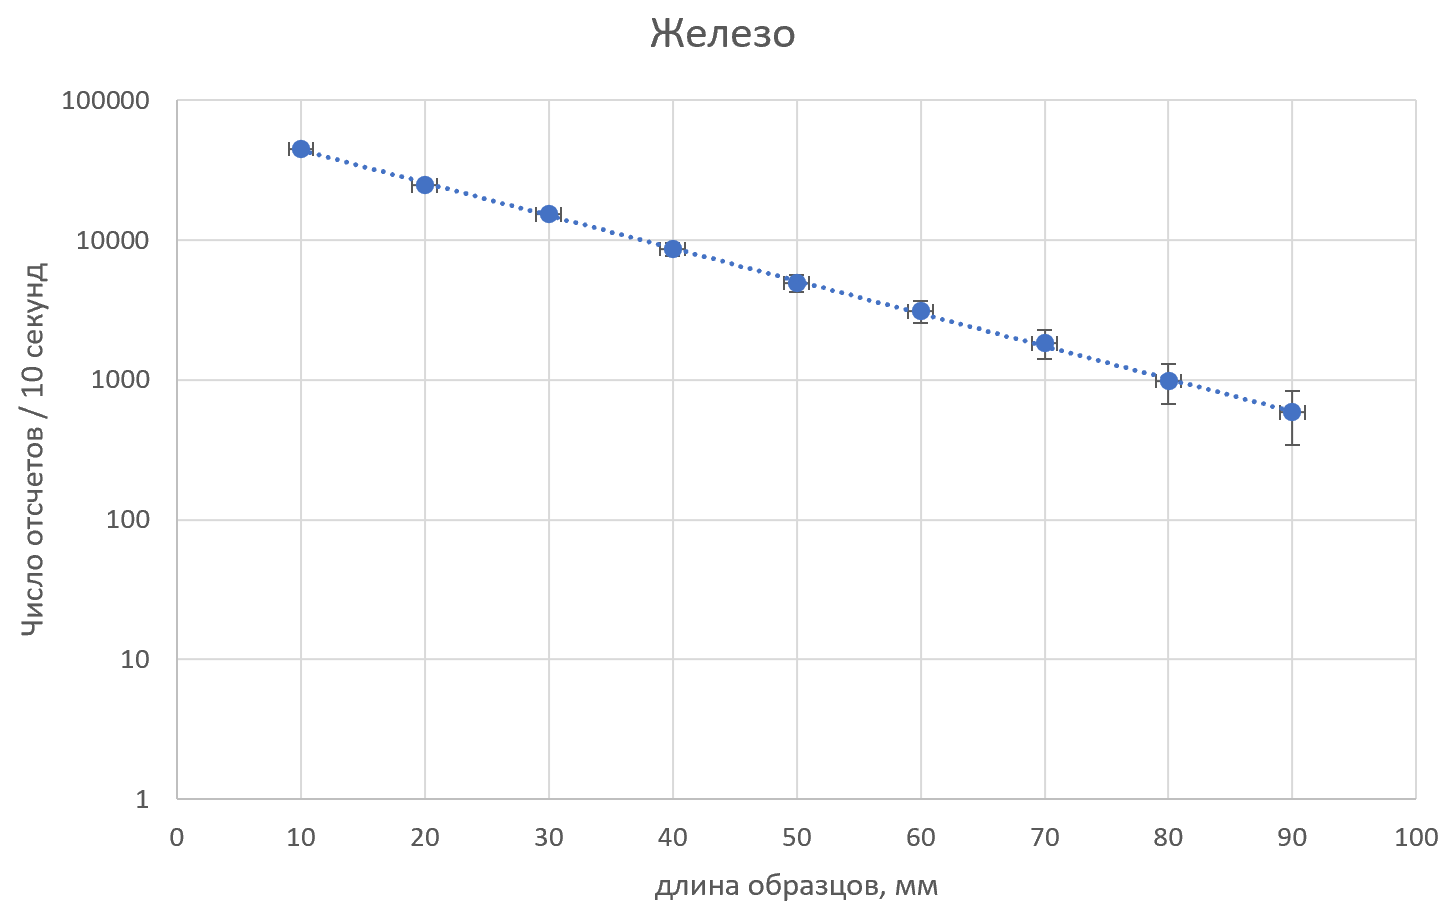
\includegraphics[scale=0.23]{10.png}
\centering
\end{figure}

.

\begin{figure}[h]
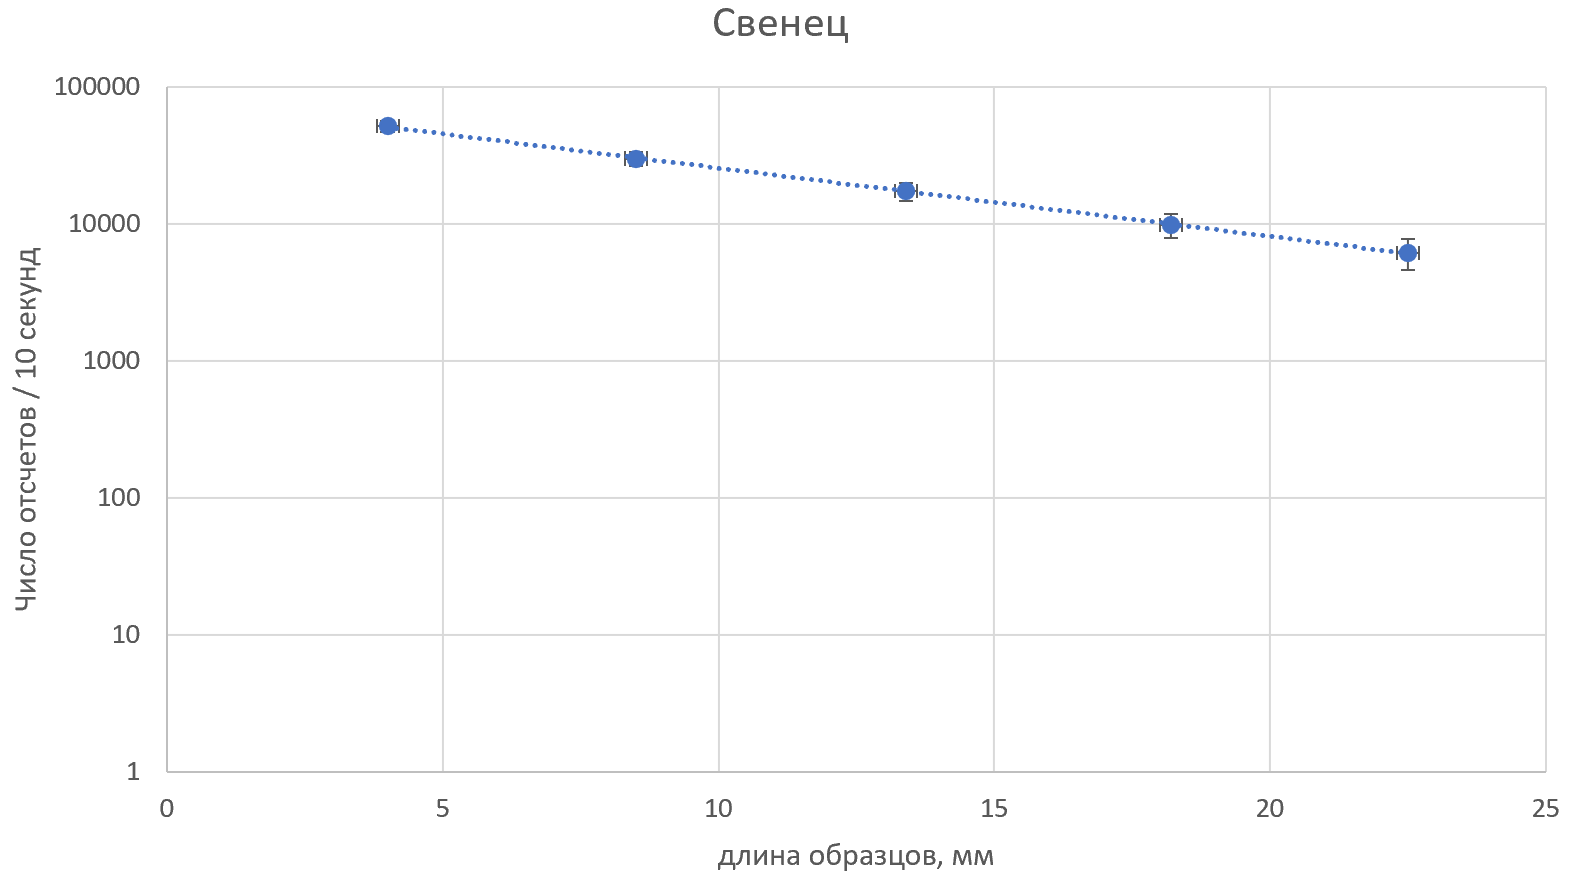
\includegraphics[scale=0.23]{20.png}
\centering
\end{figure}

.

\begin{figure}[h]
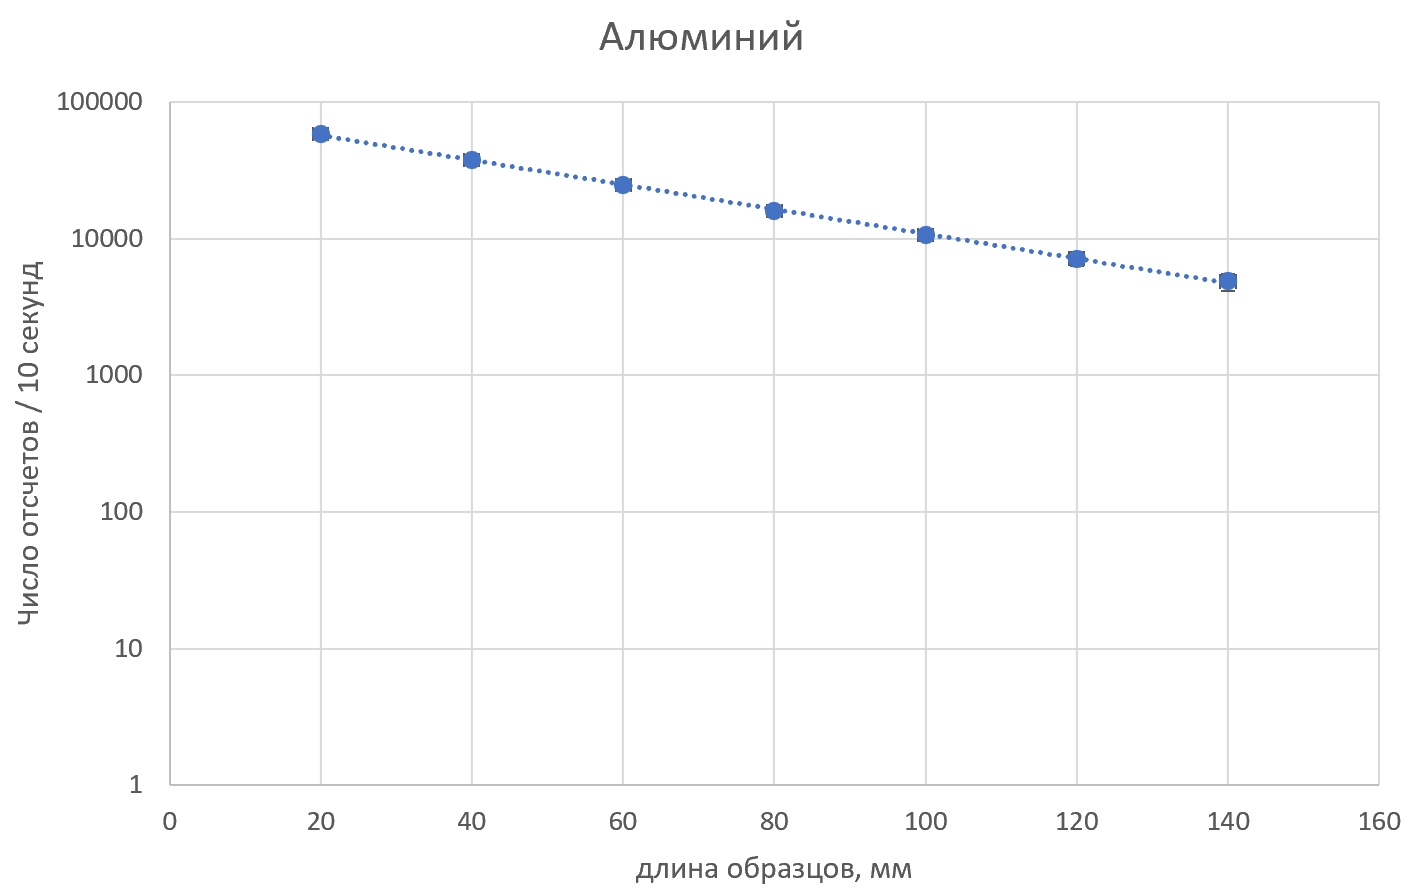
\includegraphics[scale=0.23]{30.png}
\centering
\end{figure}

\newpage

В Таблице представлены коэффициенты наклона, они же коэффициенты поглощения $\mu$, погрешность взята из МНК. По таблице в учебнике определим среднюю энергию $\gamma$-квантов в каждом опыте.

\[
\text{железо } y = (4.877 \pm 0.011) - (0.02336 \pm 0.0002) \cdot x\]
\[\text{свинец } y = (4.9102 \pm 0.0062) - (0.04991 \pm 0.00042) \cdot x\]
\[\text{алюминий } y = (4.967 \pm 0.017) - (0.01212 \pm 0.00019) \cdot x
\]

Найдем угловые коэффициенты прямых для каждой установки по МНК.

\[
	a = \frac{<x_i y_i> - < x > < y_i >}{< x_i^2> - < x_i >^2}
\]

\[
	b = < \nu_i > - a < N_i >
\]

Также рассчитаем их погрешности

\begin{equation}
	S_a^2 = \frac{< x_i^2>}{< x_i^2 > - < x_i >^2} \cdot \frac{<  b_i - b > ^2}{n - 2}
\end{equation}

Пересчитаем эти значения в коэффициент поглощения по формуле 3.

\begin{table}[h!]
\begin{tabular}{|c|c|c|c|}
\hline
   & $\mu$, $\text{см}^{-1}$ & $\sigma_\mu$, $\text{см}^{-1}$ & $E_\gamma$, МэВ \\ \hline
Pb & 1.44                    & 0.06                           & 0.60             \\ \hline
Al & 0.249                   & 0.004                          & 0.60             \\ \hline
Fe & 0.703                   & 0.010                          & 0.50             \\ \hline
\end{tabular}
\centering
\caption{Значения коэффициентов поглощения и энергия $\gamma$-квантов.}
\end{table}






%\begin{figure}[!h]
%	\centering
%	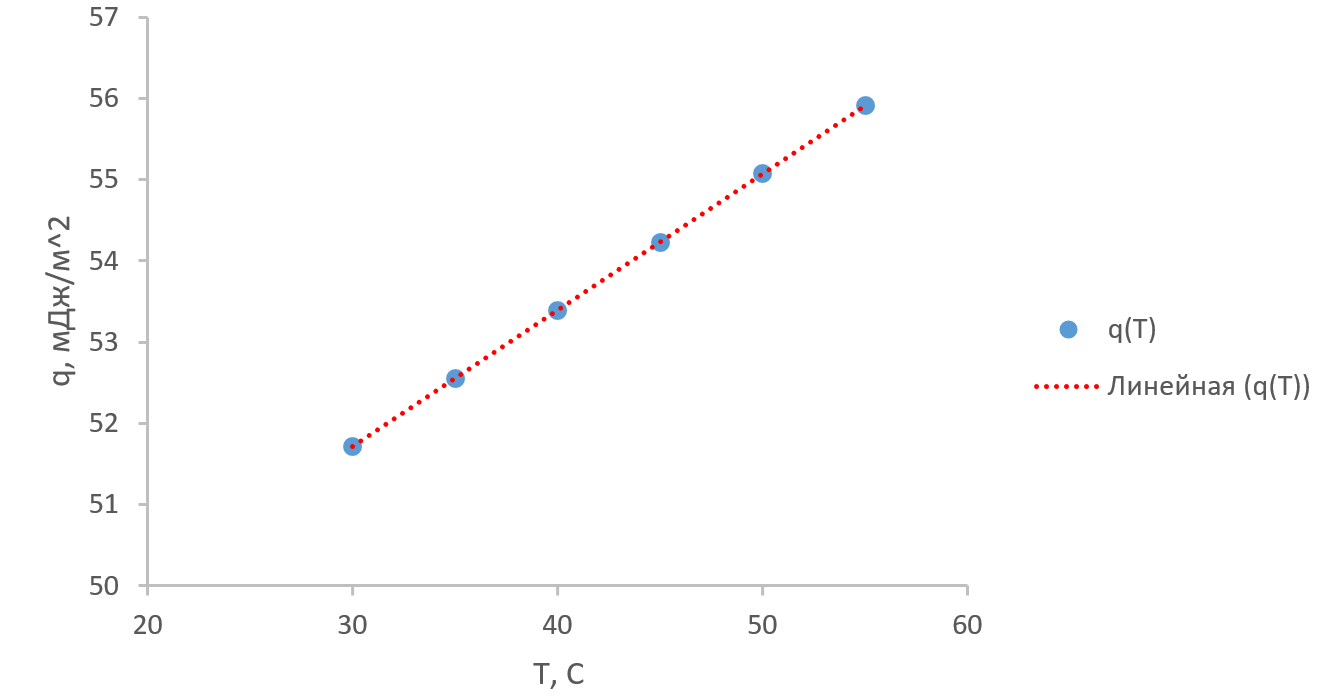
\includegraphics[width=1\textwidth]{2023-02-23_22-23-59.png}
%	\label{fig:boiler}
%\end{figure}

\section{Вывод}

Длины свободного пробега ожидаемо соответствует плотности металлов, хоть и не пропорциональна. Для алюминия и железа пропорциональность приближенно выполнена(в пределах 10$\%$) в то время как для свинца отличие существенно(20$\%$). Это говорит о большем вкладе фотоэлектрического поглощения, поскольку оно сильно зависит от заряда. В остальном, значения близки к табличным и позволяют говорить о верной постановке эксперимента. Энергия излучения совпадает с указанной для препарата на установке. 


\section{Ресурсы}

Расчет по МНК: метод-наименьших-квадратов.рф


\end{problem}
\end{document}